\section{JVM Architecture}

\index{JVM}

This section presents the details of the implementation of the JVM on
JOP. The representation of objects and the stack frame is chosen to
support JOP as a processor for real-time systems. However, since the
data structures are realized through microcode they can be easily
changed for a system with different needs.

\subsection{Runtime Data Structures}

\index{JVM!data structures}

Memory is addressed as 32-bit data, which means that memory pointers
are incremented for every four bytes. No single byte or 16-bit access
is necessary. The abstract type reference is a pointer (via a handle
indirection) to memory that represents the object or an array. The
reference is pushed on the stack before an instruction can operate on
it. A null reference is represented by the value 0.

\subsubsection{Stack Frame}

On invocation of a method, the invoker's context is saved in a newly
allocated frame on the stack. It is restored when the method returns.
The saved context consists of the following registers:

\begin{description}

\item[SP:] Immediately before invocation, the stack pointer
    points to the last argument for the called function. This
    value is reduced by the argument count (i.e. the arguments
    are consumed) and saved in the new stack frame.

\item[PC:] The pointer to the next bytecode instruction after the invoke
instruction.

\item[VP:] The pointer to the memory area on the stack that contains
the locals.

\item[CP:] The pointer to the constant pool of the class from the invoking
method.

\item[MP:] The pointer to the method structure of the invoking method.

\end{description}

SP, PC and VP are registers in JOP while CP and MP are local
variables of the JVM. \figurename~\ref{fig_jvm_stack_invoke} provides
an example of the stack before and after invoking a method. In this
example, the called method has two arguments and contains two local
variables. If the method is a virtual one, the first argument is the
reference to the object (the \emph{this}-pointer). The arguments
implicitly become locals in the called method and are accessed in the
same way as local variables. The start of the stack frame
(\emph{Frame} in the figure) needs not to be saved. It is not needed
during execution of the method or on return. To access the starting
address of the frame (e.g. for an exception) it can be calculated
with information from the method structure:

\[Frame = VP + arg\_cnt + locals\_cnt\]

\begin{figure}
    \centering
    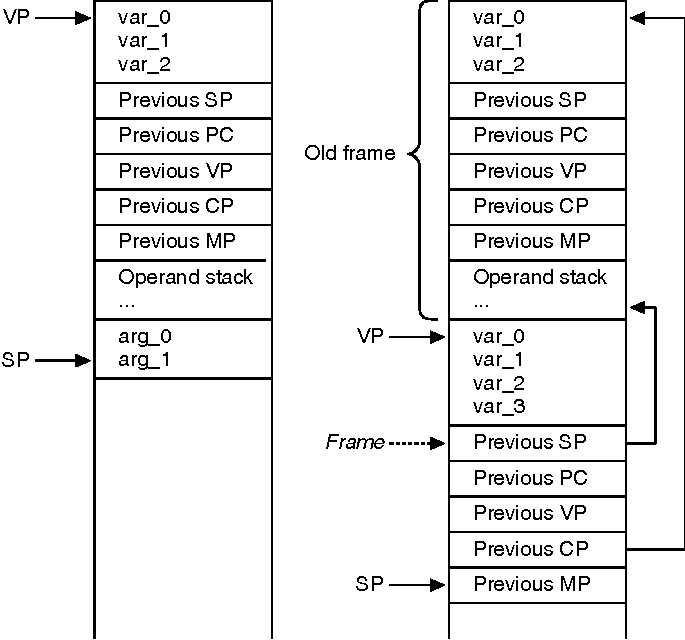
\includegraphics[scale=\picscale]{jvm/jvm_stack_invocation}
    \caption{Stack change on method invocation}
    \label{fig_jvm_stack_invoke}
\end{figure}

\subsubsection{Object Layout}

\index{object layout}

\figurename~\ref{fig_jvm_object} shows the representation of an
object in memory. The object reference points to a handle area and
the first element in the handle area points to the first instance
variable of the object. At the offset $1$ in the handle area, a
pointer is located to access class information. To speed-up method
invocation, it points directly to the method table of the objects
class instead of the beginning of the class data. The handle
indirection simplifies the implementation of a compacting GC (see
Chapter~\ref{chap:rtgc}).


\begin{figure}
    \centering
    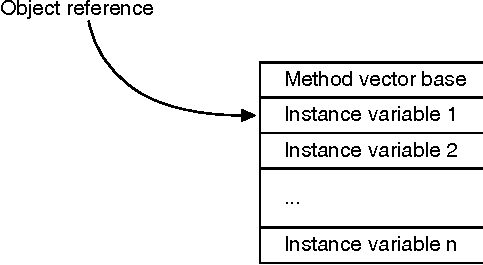
\includegraphics[scale=\picscale]{jvm/jvm_object}
    \caption{Object format}
    \label{fig_jvm_object}
\end{figure}

\subsubsection{Array Layout}

\index{array layout}

\figurename~\ref{fig_jvm_array} shows the representation of an array
in memory. The array reference points to a handle area and the first
element in the handle area points to the first element of the array.
At the offset $1$ in the handle area, the length of the array can be
found.

\begin{figure}
    \centering
    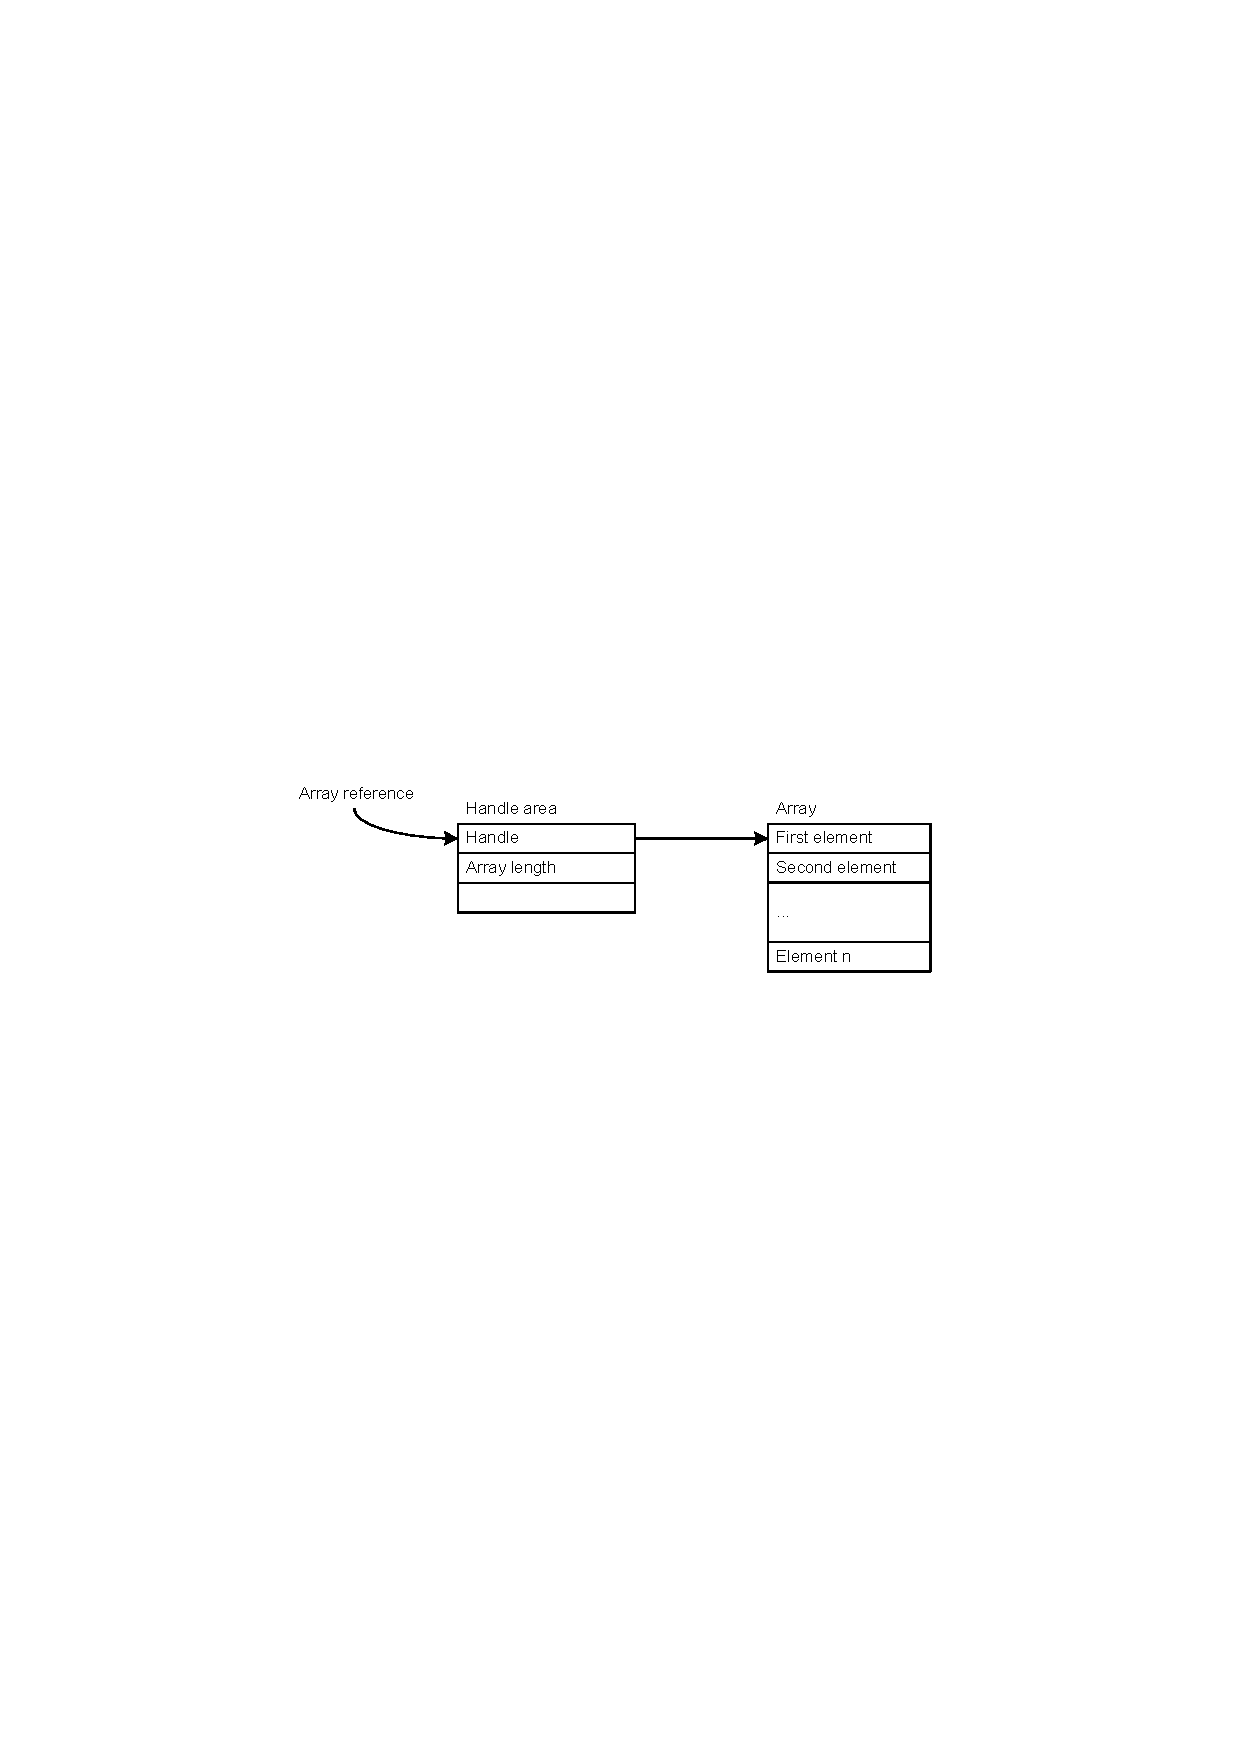
\includegraphics[scale=\picscale]{jvm/jvm_array}
    \caption{Array format}
    \label{fig_jvm_array}
\end{figure}


\subsubsection{Class Structure}

\index{class structure}


Runtime class information, as shown in Figure~\ref{fig_jvm_class},
consists of the instance size, GC info, the dispatch table for the
methods, a reference to the super class, the constant pool, and an
optional interface table. The class variables (static fields) are
located at the start of the memory to speedup access to the fields
(the constant pool index of \code{getstatic} and \code{putstatic} is
converted at class link time to the address in memory). Furthermore
all reference static fields are located in one continuous region for
simple GC root scanning. A pointer to the static primitive fields of
the class is needed for the implementation of hardware objects.

\begin{figure}
    \centering
    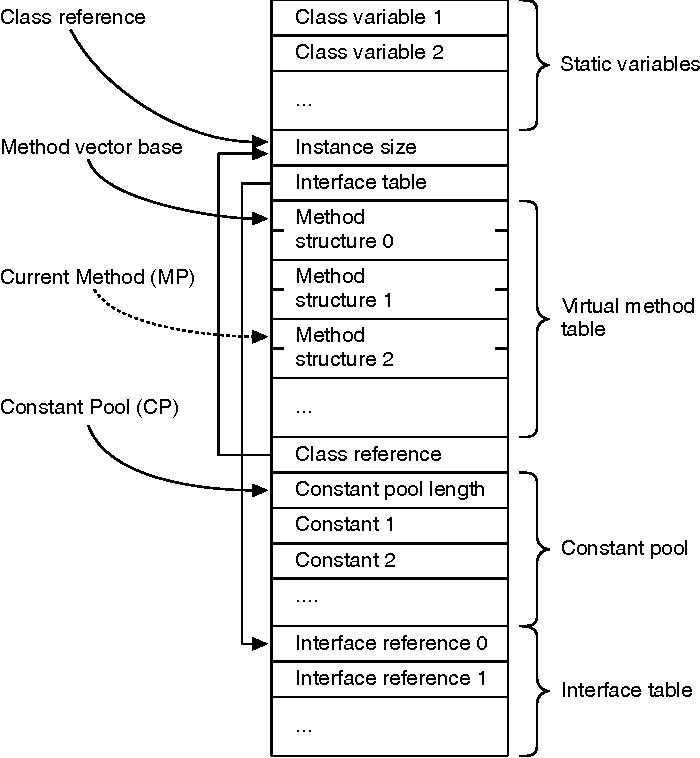
\includegraphics[scale=\picscale]{jvm/jvm_class}
    \caption{Runtime class structure}
    \label{fig_jvm_class}
\end{figure}


The class reference is obtained from the constant pool when a new
object is created. The method vector base pointer is a reference from
an object to its class (see Figure~\ref{fig_jvm_object}). It is used
on \code{invokevirtual}. The index is the argument of the bytecode to
avoid an additional memory access in invoke (the original index into
the constant pool is overwritten by the direct index at class link
time). A pointer to the method structure of the current method is
saved in the JVM variable MP. The method structure, as shown in
Figure~\ref{fig_jvm_method}, contains the starting address and length
of the method (in 32-bit words), argument and local variable count
and a pointer to the constant pool of the class. Since the constant
pool is an often accessed memory area, a pointer to it is cached in
the JVM variable CP.

\begin{figure}
    \centering
    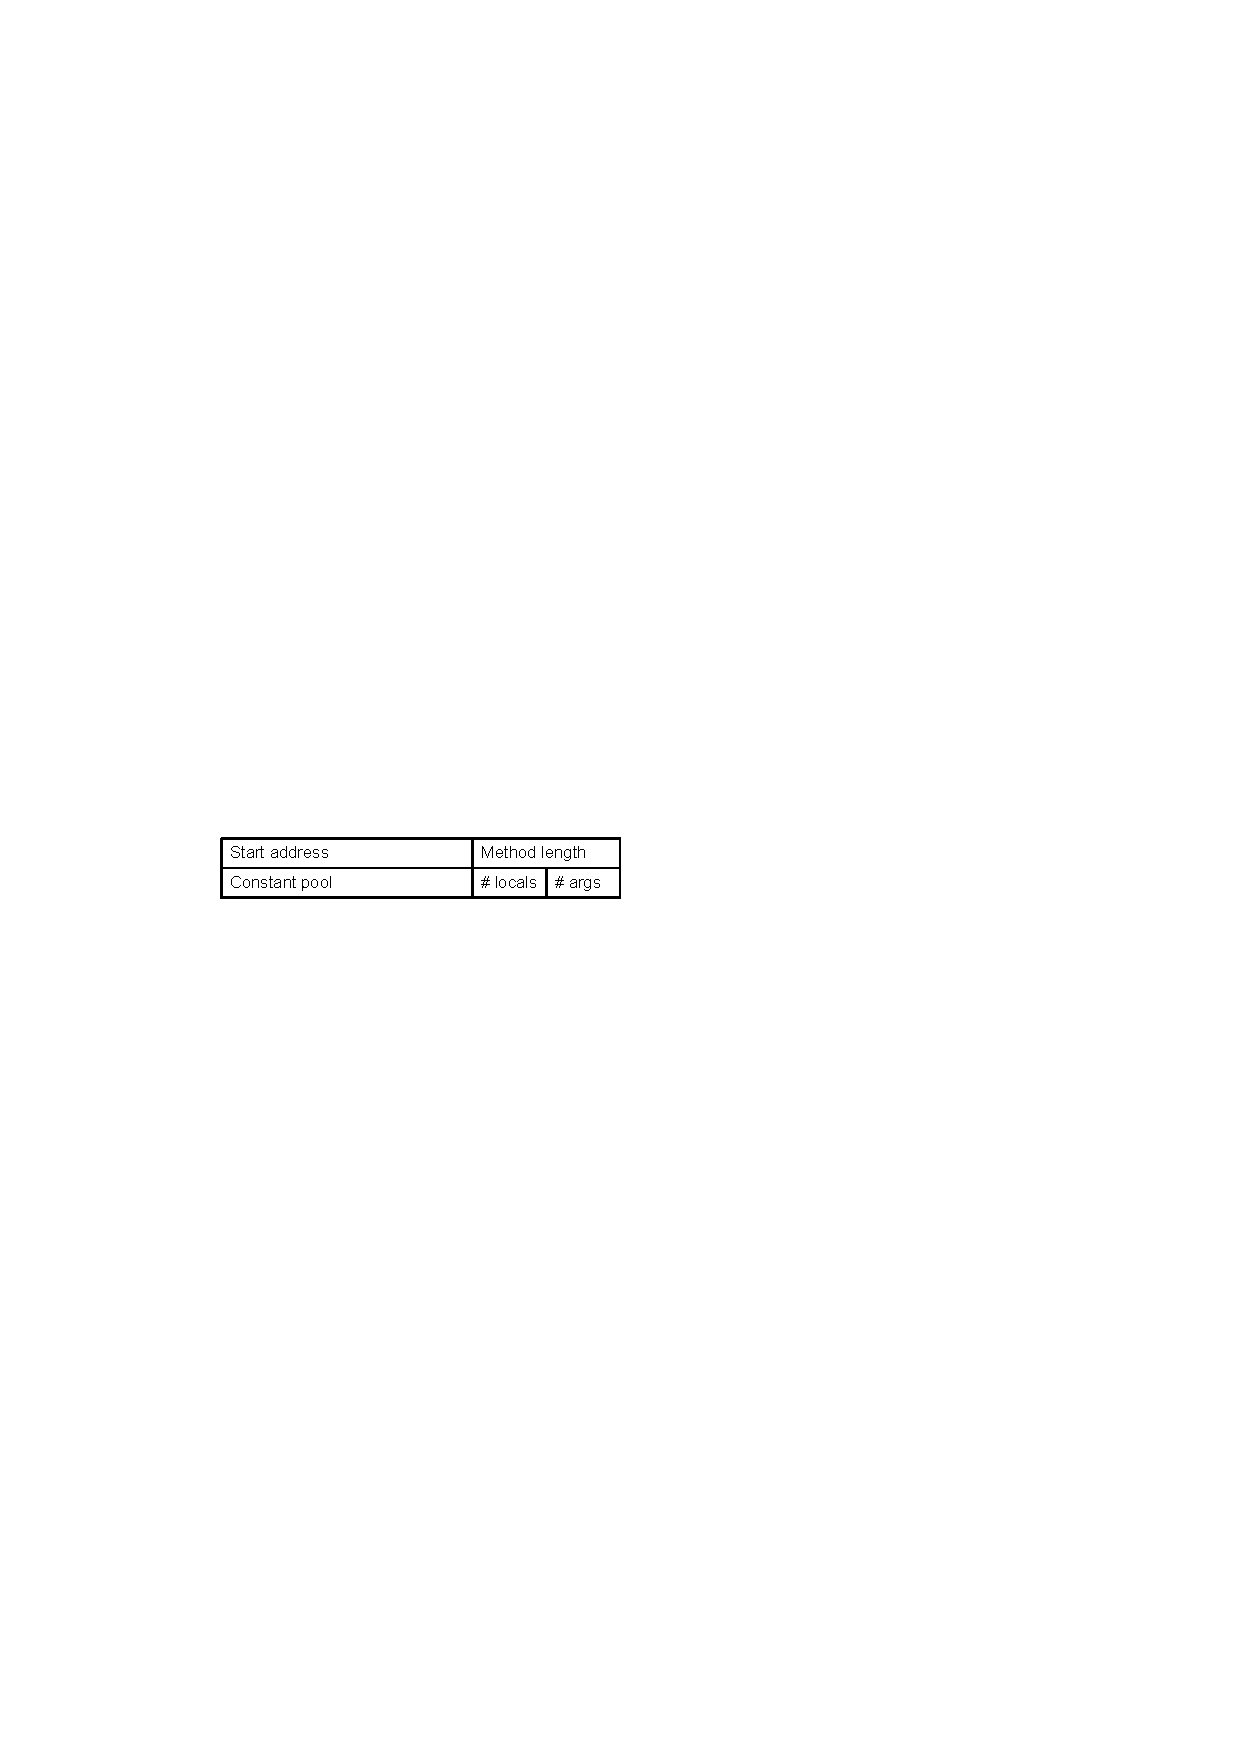
\includegraphics[scale=\picscale]{jvm/jvm_method}
    \caption{Method structure}
    \label{fig_jvm_method}
\end{figure}


The interface table contains references to the method structures of
the implementation. Only classes that implement an interface contain
this table. To avoid searching the class hierarchy on
\code{invokeinterface}, each interface method is assigned a unique
index. This arrangement provides constant execution time, but can
lead to large interface tables.

The constant pool contains various constants of a class. The entry at
index 0 is the length of the pool. All constants, which are symbolic
in the class files, are resolved during class linking. The different
constant types and their values after resolving are listed in
\tablename~\ref{tab_jvm_const_pool}. The names for the types are the
same as in the JVM specification \cite{jvm}.


\begin{table}[t]
    \centering
    \begin{tabular}{ll}
        \toprule
        Constant type &  Description \\
        \midrule
        Class &  A pointer to a class (class reference) \\
        Fieldref &   For static fields: a direct pointer to the field \\
                &   For object fields: the position relative to the object \\
                & reference \\
        Methodref &  For static methods: a direct pointer to the method structure \\
                & For virtual methods: the offset in the method table \\
                & (= index*2) and the number of arguments \\
        InterfaceMethodref &  A system wide unique index into the interface table \\
        String  & A pointer to the string object that represents the string \\
                & constant \\
        Integer & The constant value \\
        Float   & The constant value \\
        Long    & This constant value spans two entries in the constant pool \\
        Double  & Same as for long constants \\
        NameAndType & Not used \\
        Utf8    & Not used \\
        \bottomrule
    \end{tabular}
    \caption{Constant pool entries}
    \label{tab_jvm_const_pool}
\end{table}

\subsection{Class Initialization}
\label{para:restrict:clinit}

\index{JVM!class initialization}


According to \cite{jvm} the static initializers of a class C are
executed immediately before one of the following occurs: (i) an
instance of C is created; (ii) a static method of C is invoked or
(iii) a static field of C is used or assigned. The issue with this
definition is that it is not allowed to invoke the static
initializers at JVM startup and it is not so obvious when it gets
invoked.

It follows that the bytecodes \code{getstatic}, \code{putstatic},
\code{invokestatic} and \code{new} can lead to class initialization
and the possibility of high WCET values. In the JVM, it is necessary
to check every execution of these bytecodes if the class is already
initialized. This leads to a loss of performance and is violated in
some existing implementations of the JVM. For example, the first
version of CACAO \cite{cacao} invokes the static initializer of a
class at compilation time. Listing~\ref{lst:retrict:clinit} shows an
example of this problem.

\cmd{JOPizer} tries to find a correct order of the class initializers
and puts this list into the application file. If a circular
dependency is detected the application will not be built. The class
initializers are invoked at JVM startup.

\begin{lstlisting}[float=t,caption={Class initialization can occur very late},
label=lst:retrict:clinit]
    public class Problem {

        private static Abc a;
        public static int cnt; // implicitly set to 0

        static {
            // do some class initializaion
            a = new Abc();  //even this is ok.
        }

        public Problem() {
            ++cnt;
        }
    }

    // anywhere in some other class, in situation,
    // when no instance of Problem has been created
    // the following code can lead to
    // the execution of the initializer
    int nrOfProblems = Problem.cnt;
\end{lstlisting}

\subsection{Synchronization}

Synchronization is possible with methods and on code blocks. Each
object has a monitor associated with it and there are two different
ways to gain and release ownership of a monitor. Bytecodes
\code{monitorenter} and \code{monitorexit} explicitly handle
synchronization. In other cases, synchronized methods are marked in
the class file with the access flags. This means that all bytecodes
for method invocation and return must check this access flag. This
results in an unnecessary overhead on methods without
synchronization. It would be preferable to encapsulate the bytecode
of synchronized methods with bytecodes \code{monitorenter} and
\code{monitorexit}. This solution is used in Suns picoJava-II
\cite{pjProgRef}. The code is manipulated in the class loader. Two
different ways of coding synchronization, in the bytecode stream and
as access flags, are inconsistent. With \cmd{JOPizer} the same
manipulation of the methods is performed to wrap the method code in a
synchronized block when the method is defined synchronized.
